\section{Results}

Implementation of our approach is provided in the \R\ package
\href{https://dajmcdon.github.io/rtestim/}{\texttt{rtestim}}. All experiments
are run in \R\ version 4.3.1 on a MacBook with an Apple M1 Pro chip
and 32GB RAM running under macOS Sonoma 14.0. The \R\ packages used for
simulation and real-data application are \texttt{EpiEstim 2.2-4},
\texttt{EpiLPS 1.2.0}, and \texttt{rtestim 0.0.4}. 

\subsection{Synthetic experiments}

We simulate four scenarios of the time-varying effective reproduction number,
intended to mimic different epidemics. The first two scenarios are rapidly controlled by intervention, where the $\calR(t)$ consists
of one discontinuity and two segments. Scenario 1 has constant $\calR(t)$ before
and after an intervention, while Scenario 2 grows exponentially, then decays.
The other two scenarios are more complicated, where more waves
are involved. Scenario 3 has four linear segments with three discontinuities,
which reflect the effect of an intervention, resurgence to rapid transmission,
and finally suppression of the epidemic. Scenario 4 involves sinusoidal waves
throughout the epidemic.
The first three scenarios and the last scenario are motivated by
\cite{parag2021improved} and \cite{gressani2022epilps} respectively. 
We name the four scenarios as \textit{(1) piecewise constant}, \textit{(2) 
piecewise exponential}, \textit{(3) piecewise linear}, and \textit{(4) periodic} 
lines or curves respectively. 



In all cases, the times of observation are regular, and epidemics are of
length $n=300$. Specifically, in Scenario 1, $\calR_t = 2, 0.8$ before and after
$t=70$. In Scenario 2, $\calR_t$ increases and decreases exponentially with
rates $0.015, 0.005$ pre and post $t=50$. 
In Scenario 3, $\calR_t$ is piecewise linear with four discontinuous segments following 
\begin{align*}
    \calR(t) = & \lr{2.5 - \frac{0.5}{59}\lr{t-1}} \boldsymbol{1}_{[1,60]}(t)
     + \lr{0.8 - \frac{0.2}{49}\lr{t-61}} \boldsymbol{1}_{(60,110]}(t) \\
    & + \lr{1.7 + \frac{0.3}{39}\lr{t-111}} \boldsymbol{1}_{(110,150]}(t)
     + \lr{0.9 - \frac{0.4}{149}\lr{t-151}} \boldsymbol{1}_{(150,300]}(t),
\end{align*}
where $\boldsymbol{1}_{A}(t) = 1$, if $t\in A$, and $\boldsymbol{1}_{A}(t)=0$ otherwise. 
In Scenario 4, $\calR_t$ is realization of the 
continuous, periodic curve generated by the function $$\calR(t) = 0.2 \big(
\lr{\sin(\pi t/12) + 1} + \lr{2 \sin\lr{\pi t / 6} + 2} + \lr{3
\sin(\pi t / 1.2) + 3}\big),$$ evaluated at equally spaced points $t\in [0,10]$. 
These settings are illustrated in the left column of \autoref{fig:samples}.


We assume that the serial interval follows the Gamma distribution with fixed
shapes and scales $(3,3)$, $(2.5,2.5)$, $(3.5,3.5)$ and $(3.5,3.5)$ for
Scenarios 1--4 respectively. We initialize all epidemics with $y_1=2$ cases and
generating for $t=2,\ldots,300$. We compute the expected incidence $\Lambda_t$
using the renewal equation, and generate the incident infections from the
Poisson distribution $y_t\sim \textrm{Pois}(\Lambda_t)$. To verify the
performance of our model under the violation of this distributional assumption,
we also generate incident infections using the negative Binomial distribution
with dispersion size 5, i.e., $y_t\sim \textrm{NB}(\Lambda_t,\
\textrm{size}=5)$. For each setting, we generate 50 random samples, resulting in
400 total experiments. An example of each effective reproduction number scenario
with a single corresponding Poisson and negative Binomial sample incidence
sequences is displayed in \autoref{fig:samples}. 

\begin{figure}[!ht]
  \centering
  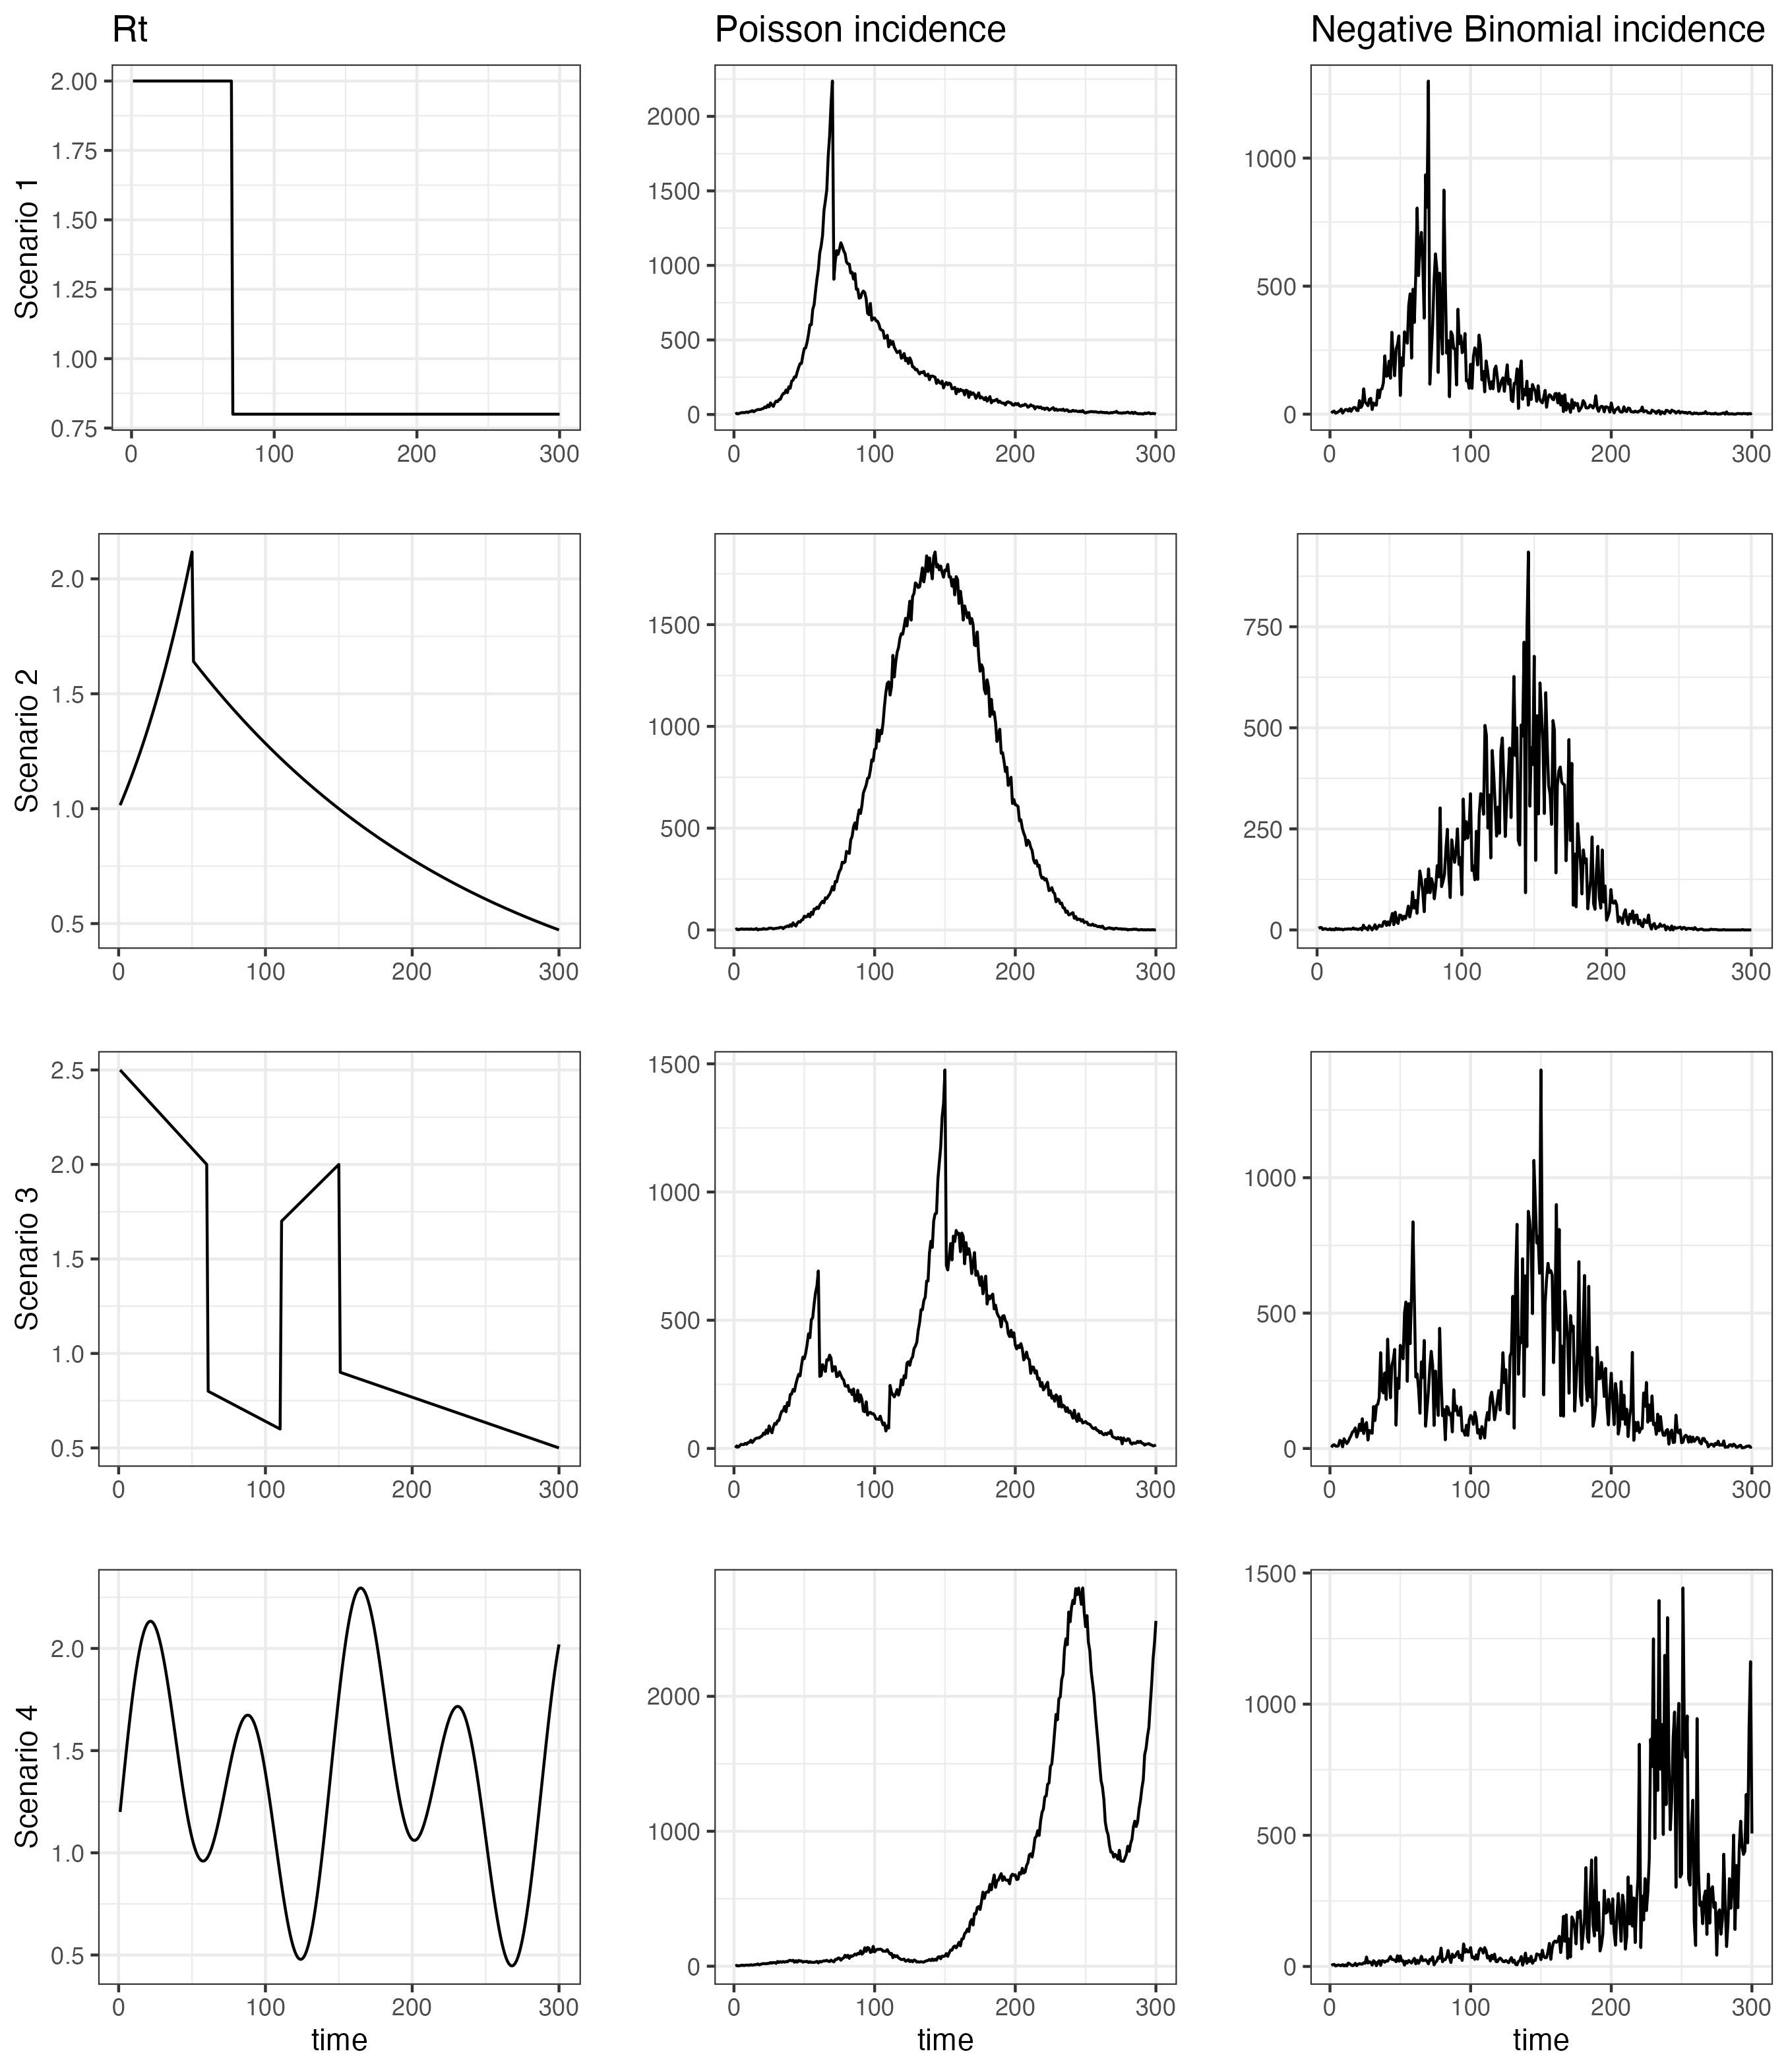
\includegraphics[width=.8\textwidth]{fig/plot_samples.png}
  \caption{The effective reproduction numbers (left column) and corresponding
  sample incident cases drawn from a  Poisson (middle column) or negative
  Binomial (right column) distribution. The rows correspond to the four
  $\calR_t$ settings.} 
  \label{fig:samples}
\end{figure}

We compare \RtEstim\ to \EpiEstim\ and \EpiLPS. Unfortunately,
\texttt{EpiFilter} frequently fails to converge due to the large incident counts
in these settings, so we are unable to include its results. \EpiEstim\ estimates
the posterior distribution of the effective reproduction number given a Gamma
prior and Poisson distributed observations
over a trailing window, under the assumption that the effective reproduction number is
constant during that window. A larger window averages out more
fluctuations,
leading to smoother estimates, whereas, a shorter sliding window is more
responsive to sudden spikes or declines. We tried the default, a weekly sliding
window, as well as a monthly window. However, since neither considerably
outperforms the other across all scenarios, we defer the monthly results to the
supplementary document. \EpiLPS\ is another Bayesian approach that estimates P-splines
based on the Laplace approximation to the conditional posterior with negative
Binomial likelihood. For \RtEstim\ on the four scenarios respectively, we
estimate (1) piecewise constant $k=0$, (2) piecewise linear \& cubic $k=1,3$,
(3) piecewise linear $k=1$ and (4) piecewise cubic polynomials $k=3$. In each
case, we examine a grid of 50 $\lambda$ values, selecting the best using 10-fold
cross validation. For all models and problems, we use the same serial interval
distribution for estimation that was used to create the data. 


To measure estimation accuracy, we compare $\widehat{\calR}$ to $\calR$ using
the Kullback-Leibler (KL) divergence. We use the KL divergence for the
Poisson distribution (summed over across all $t$) to measure the accuracy
of the $\calR_t$ estimates 
$$D_{KL}(\calR \parallel \widehat{\calR}) = \sum_{t=1}^n w_t \lr{\calR_t
\log\left(\frac{\calR_t} {\widehat{\calR}_t}\right) + \widehat{\calR}_t -
{\calR}_t},$$ where $\calR = \left\{ \calR_t \right\}_{t=1}^n$ and $w_t = \eta_t
/ \sum_t \eta_t$ is the rescaled total infectiousness. To fairly compare across
methods, we drop the estimates during the first week because estimates from
\EpiEstim\ do not begin until $t=8$ (using a weekly window). KL divergence is
more appropriate for measuring accuracy because it connects directly to the
Poisson likelihood used to generate the data, whereas standard measures like the
mean-squared error correspond to Gaussian likelihood. Using Poisson likelihood
has the effect of increasing the relative cost of mistakes when $\Lambda_t$ is
small. Other details of the experimental settings are deferred to the 
supplementary document. 


\subsection{Results for synthetic data}

\RtEstim\ overall outperforms \EpiEstim\ and \EpiLPS\ in the experimental study.
\autoref{fig:kl-res} visualizes the KL divergence across the three models. Under
both Poisson and negative Binomial distributions, \RtEstim\ is easily the most
accurate for Scenarios 1 and 3: the median of KL divergence is much lower and
the boxes frequently fail to overlap indicating better performance than the
other two methods across all 50 simulations. The advantage is less pronounced
for the negative Binomial configuration, but still obvious.
\RtEstim\ and \EpiLPS\ have similar performance in Scenarios 2 and 4. For the
Poisson case, \RtEstim\ and \EpiLPS\ both have very small KL scores, which are
very close to zero. In Scenario 4, \RtEstim\ is slightly better for Poisson and
\EpiLPS\ is better for negative Binomial, but the boxes largely overlap each
other. \EpiLPS\ has a slightly lower median and a smaller IQR in Scenario 2 for
the negative Binomial case. Both smoothness choices for \RtEstim\ in Scenario 2
perform similarly across noise distributions, implying good performance under model misspecification. We will examine a single realization of each
experiment to investigate these global conclusions in more detail.

\begin{figure}[!ht]
  \centering
  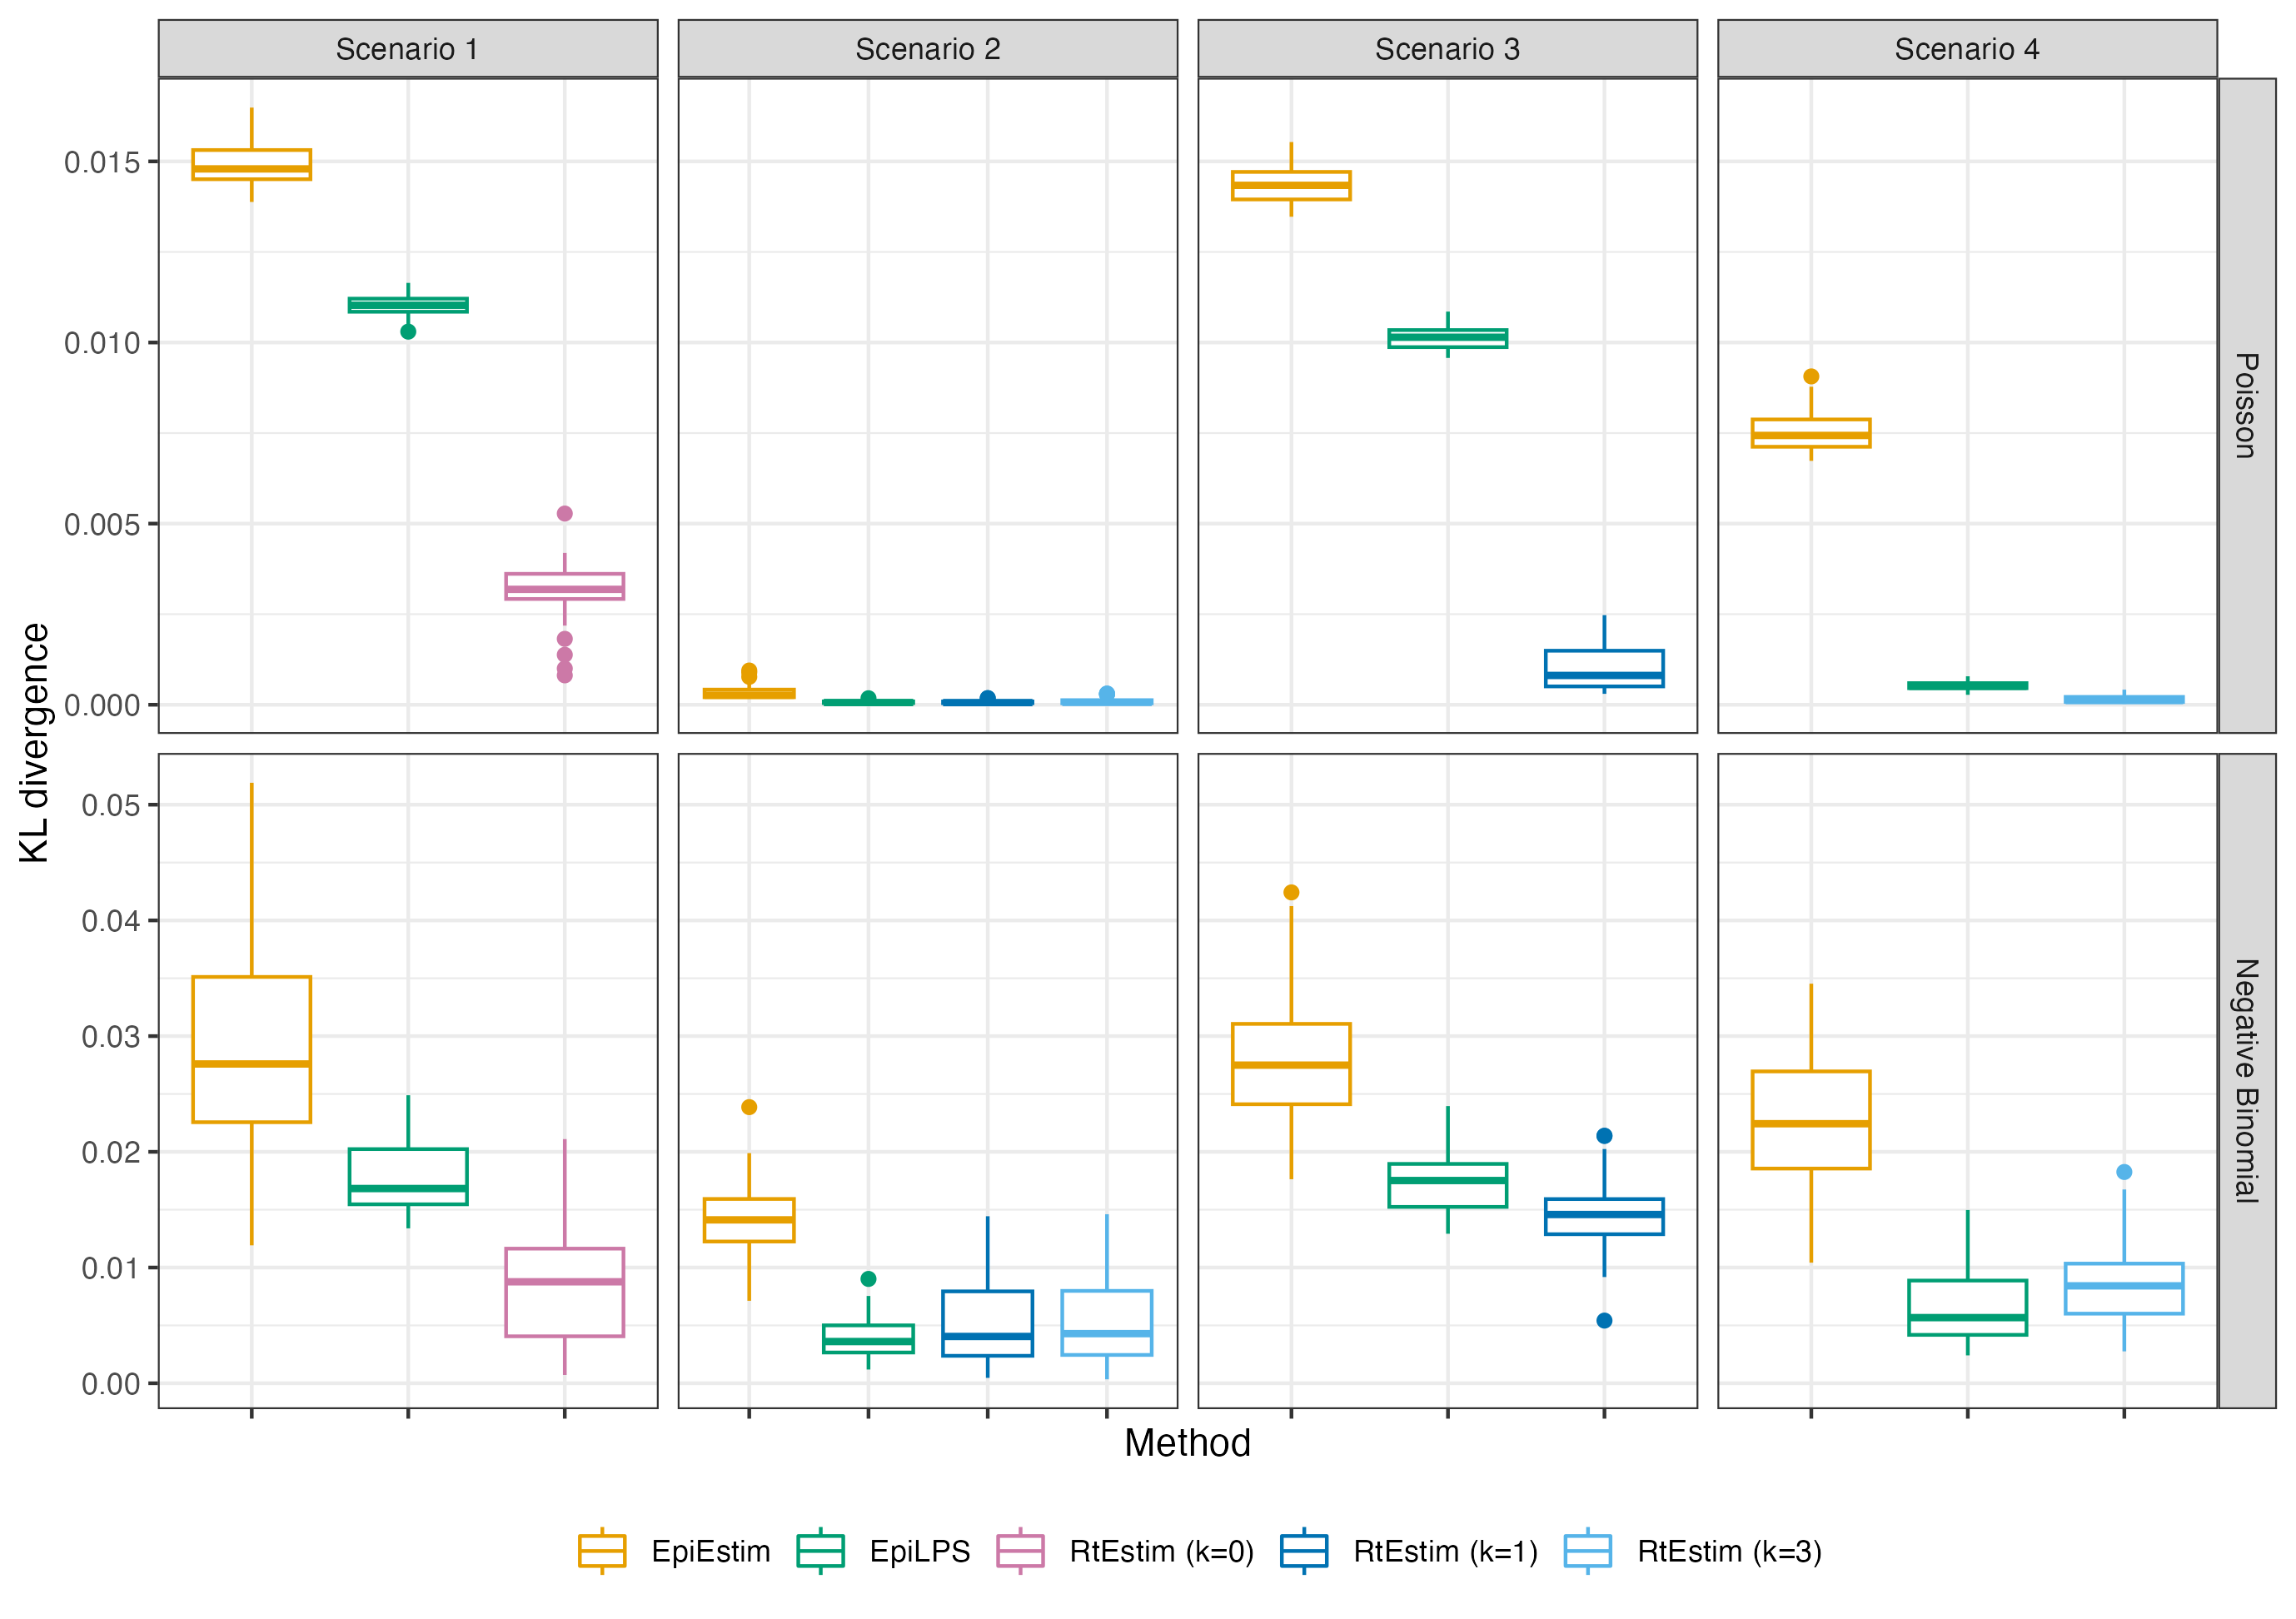
\includegraphics[width=.99\textwidth]{fig/KL_no_outlier.png}
  \caption{Boxplot of KL divergence between the estimated 
  $\hat{\calR}_t$ and the true $\calR_t$ across 50 random samples for 
  each approach given Poisson incidence \textit{(in top panels)} and negative 
  Binomial incidence \textit{(in bottom panels)} respectively.  
  Outliers are excluded.} 
  \label{fig:kl-res}
\end{figure}

\autoref{fig:pois-est} shows one realization for the estimated effective reproduction
number under the Poisson generative model for all four scenarios. Compared to
\EpiEstim\ and \EpiLPS, which have rather severe difficulties at the beginning
of the time series, \RtEstim\ estimates are more accurate---they nearly
overlap with the true values---without suffering from the initialization
problem. Scenario
1 is the simplest case with only one knot and two constant segments. Besides the
edge problem, \EpiEstim\ and \EpiLPS\ produce ``smooth'' estimated curves that
are continuous at the changepoint, which results in large mistakes in that
neighbourhood. Since the piecewise constant \RtEstim\ estimator does not force
any smoothness in $\calR_t$, it easily captures the sharp change. 
Scenario 2 is relatively easy for all methods, except at the changepoint 
occurring at the end of the exponential growth. Although the truth is
likely best represented with a discontinuous piecewise cubic curve, the actual
curvature is so gentle that linear estimation ($k=1$) appears potentially
reasonable. However,
\RtEstim\ has difficulty recovering the acute rise in the
growth phase because it enforces continuity at the changepoint. 

\begin{figure}[!ht]
  \centering
  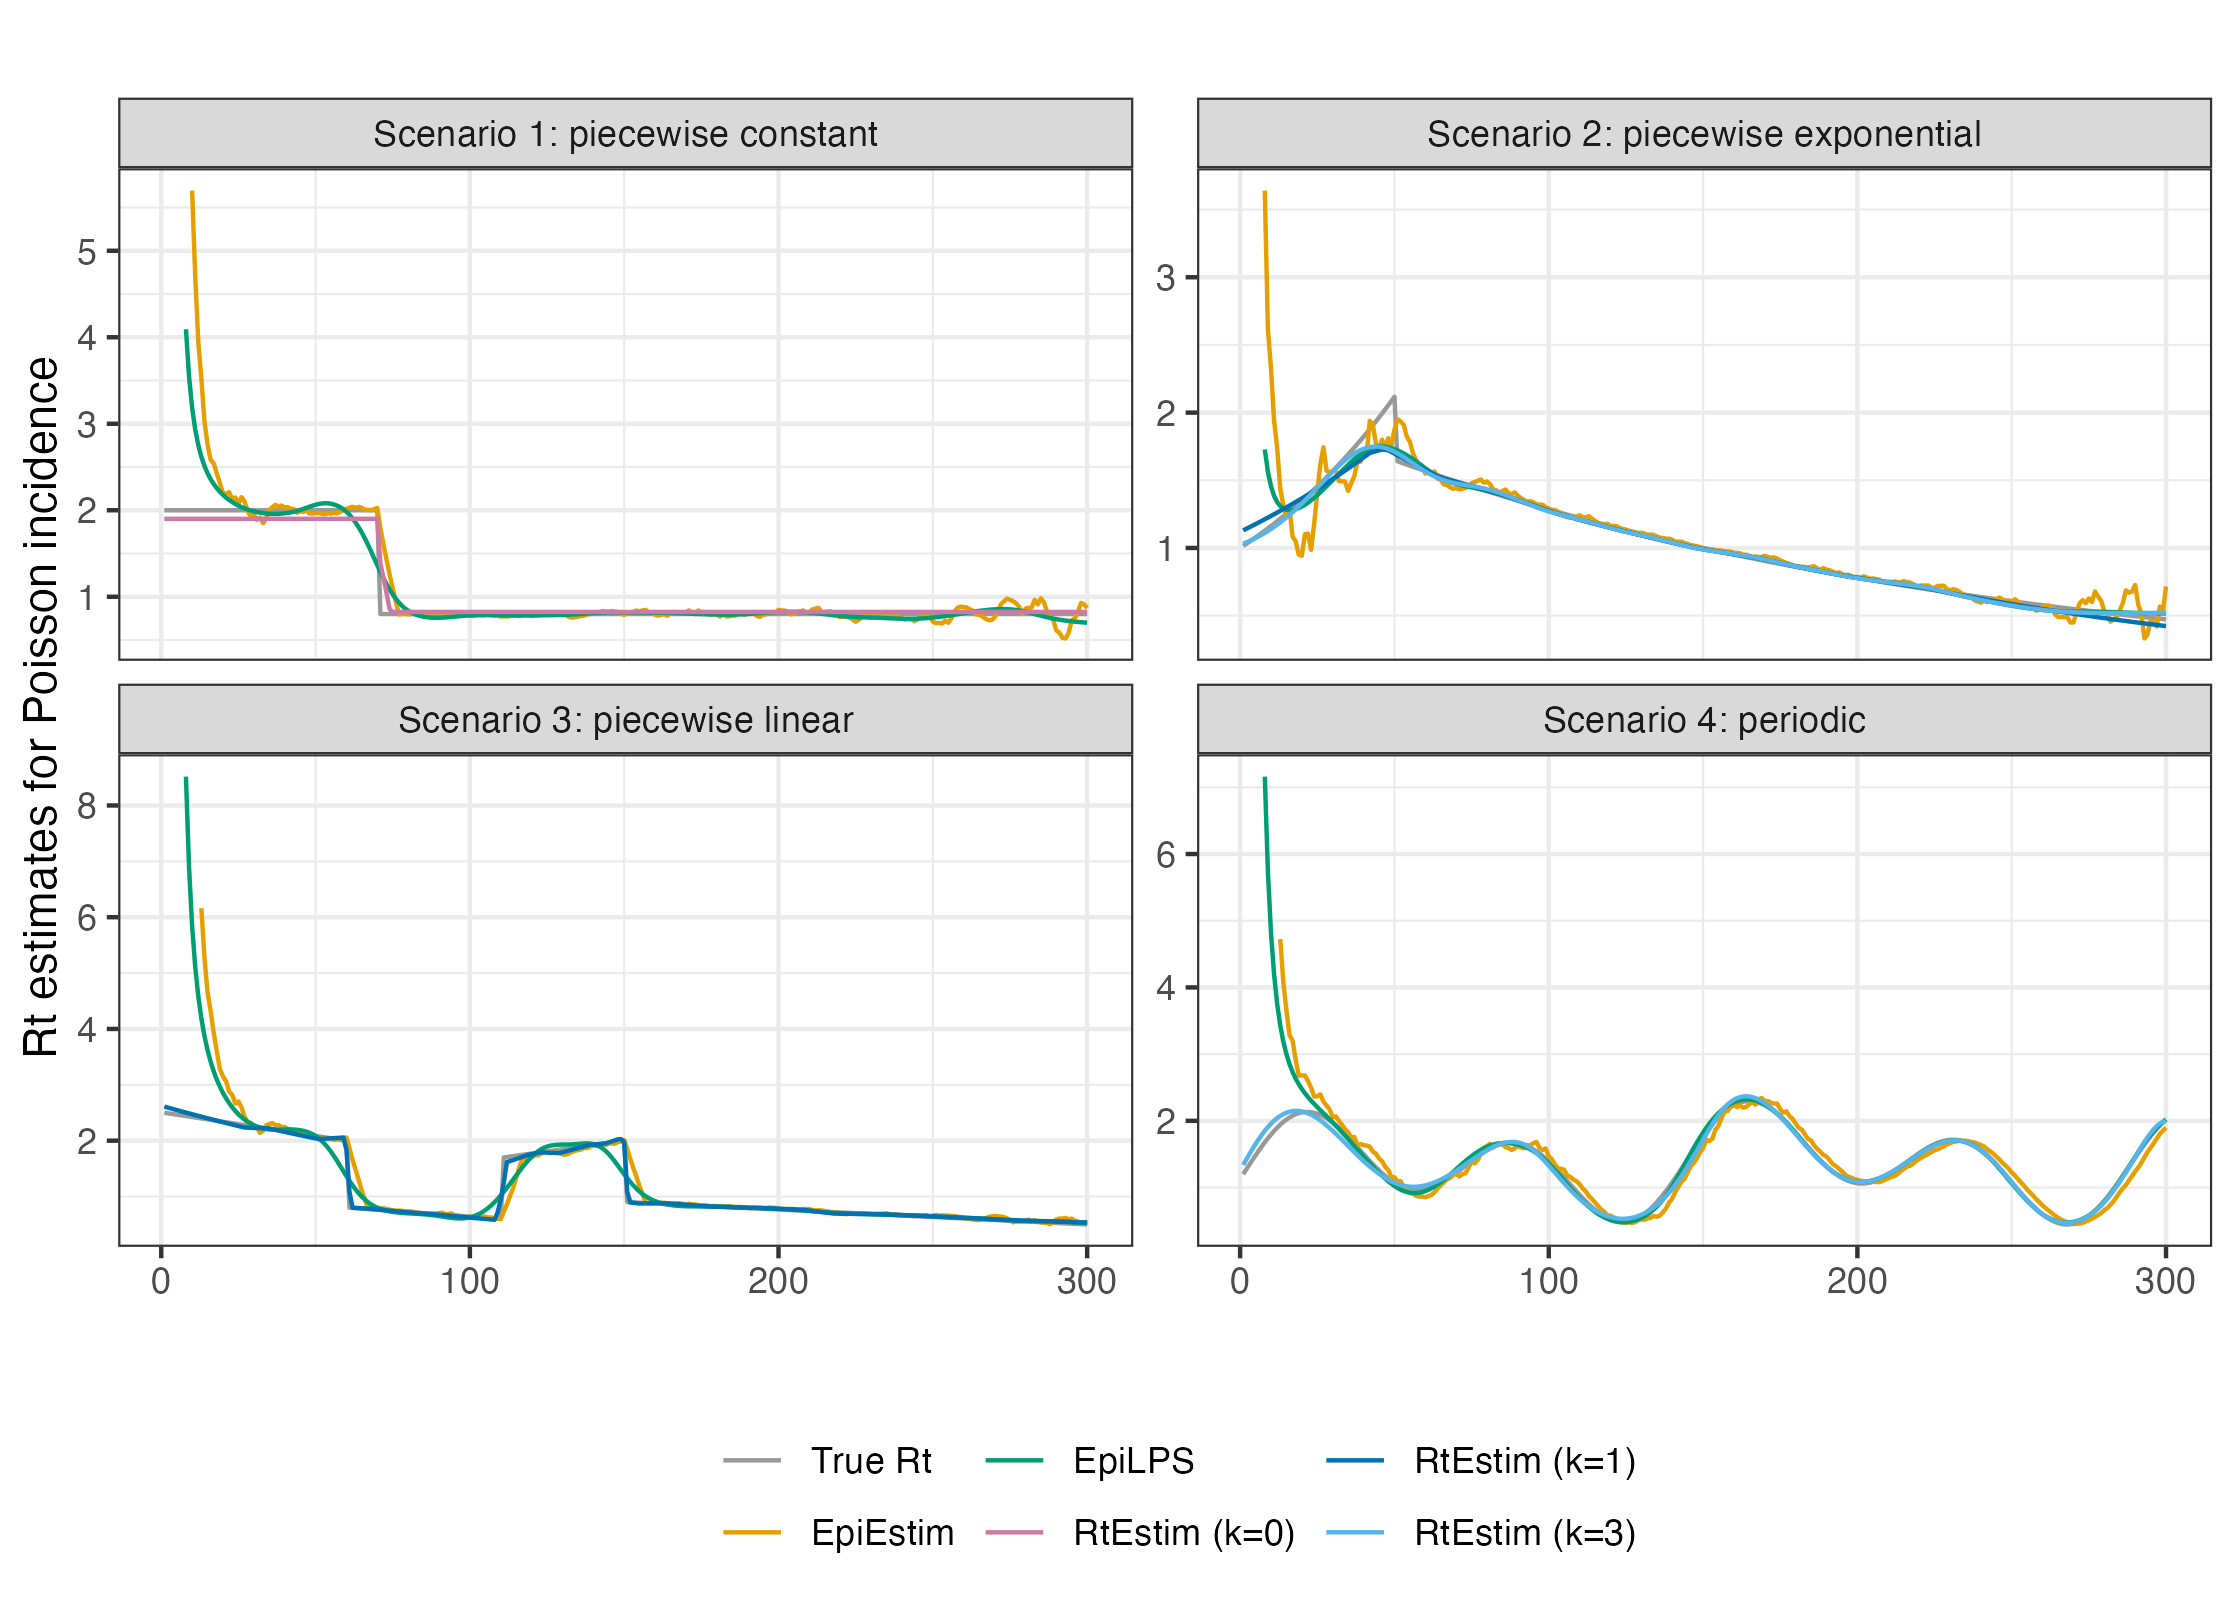
\includegraphics[width=.99\textwidth]{fig/Pois-res-plot.png}
  \caption{Example of effective reproduction number estimation for Poisson observations.}
  \label{fig:pois-est}
\end{figure}

To investigate the performance when the Poisson assumption (imposed by both
\RtEstim\ and \EpiEstim) is violated, we also examine estimation accuracy with
negative Binomial data. \autoref{fig:nb-est} displays a realization, analogous
to the previous case, for all methods and scenarios. \RtEstim\ has more
difficulty relative to the Poisson setting, especially at the beginning of the
outbreak. This is most pronounced in Scenario 4, where \RtEstim\ is overly
smooth, except in the last wave. In Scenario 2, \RtEstim\ successfully captures
the changepoint, but suffers from the same discontinuity problem as in the
Poisson setting. In Scenario 3, the piecewise linear version of \RtEstim\
recovers the curvature of $\calR_t$ well, but is less accurate than in the
Poisson case.

\begin{figure}[!ht]
  \centering
  \includegraphics*[width=.99\textwidth]{fig/NB-res-plot.png}
  \caption{Example of effective reproduction number estimation for negative
  Binomial obsersations.}
  \label{fig:nb-est}
\end{figure}

Finally, it is important to provide a brief comparison of the running times of
all three models across the $8$ experimental settings. We find that almost all
models across all experiments complete within $10$ seconds. \RtEstim\ generally
takes the longest, due to a relatively large number of estimates---$50$ values
of $\lambda$ and $10$ folds of cross validation require $550$ estimates---while
other models run only a single time for a fixed setting of hyperparameters per
experiment. Additional results on timing comparisons are deferred to the
supplementary document. 


\subsection{Real-data results: Covid-19 incident cases in British Columbia}

We implement \RtEstim\ on Covid-19 confirmed incident cases in British Columbia
(B.C.) as reported on May 18, 2023 (visualized in \autoref{fig:covid-data}) by
the B.C.\ Centre for Disease Control \citep{covidbc}. We use the gamma distribution with shape
$2.5$ and scale $2.5$ to approximate the serial interval function, which is
similar to empirical estimates~\citep{lehtinen2021relationship}. 

\begin{figure}[!ht]
  \centering
  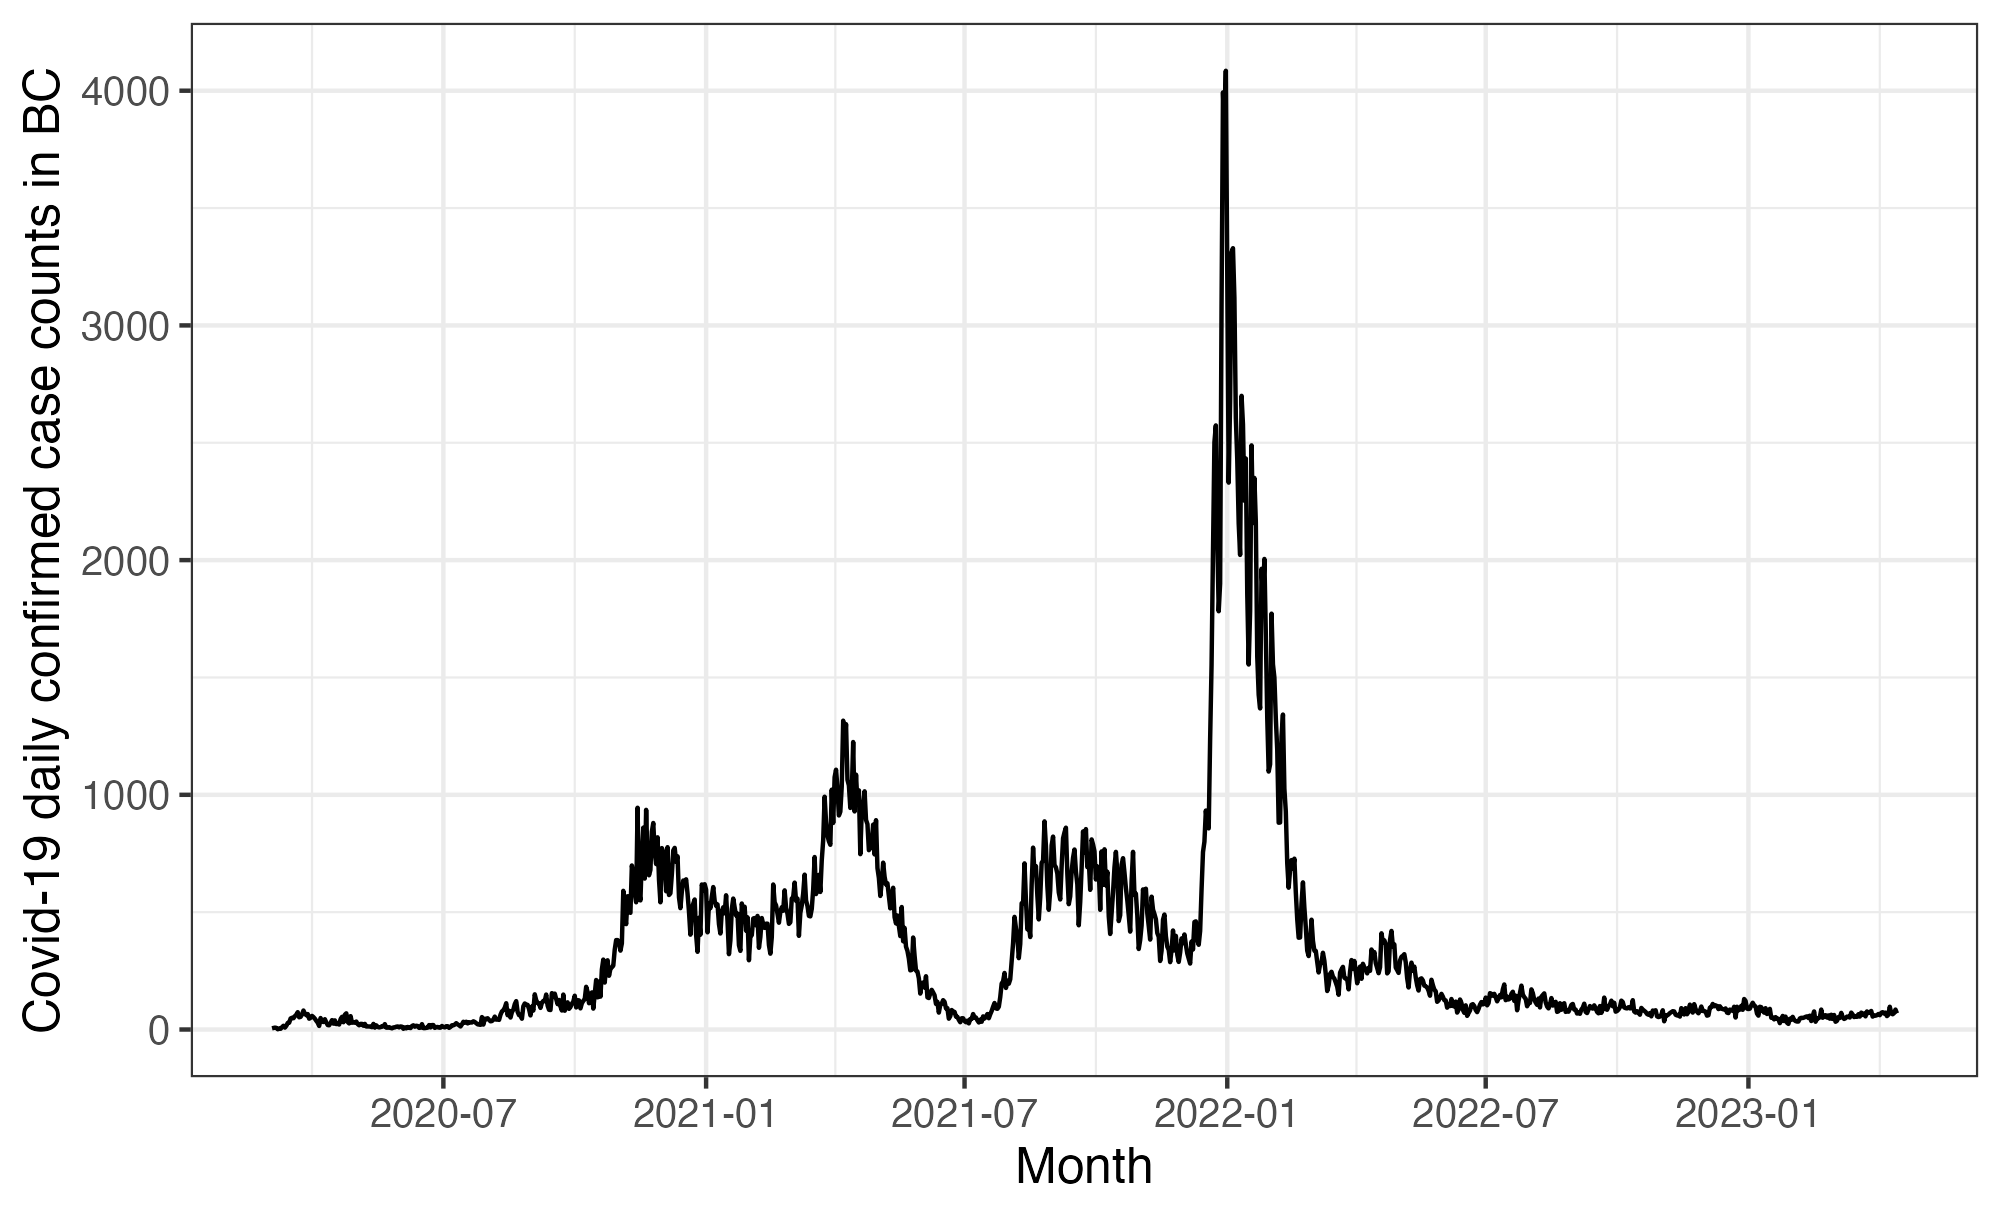
\includegraphics[width=0.9\textwidth]{fig/covid_dat.png}
  \caption{Covid-19 daily confirmed incident cases between March 1st, 
  2020 and April 15th, 2023 in British Columbia, Canada.} 
  \label{fig:covid-data}
\end{figure} 

Considering the first, second, and third polynomial degrees, $\widehat{\calR}_t$
for Covid-19 in British Columbia (illustrated in \autoref{fig:covid-rt}) is
always less than $3$ except at the very early stage, which means that one
distinct infected individuals on average infects less than three other
individuals in the population. Examining three different settings for $k$, the
temporal evolution of $\widehat{\calR}$ (across all regularization levels
$\lambda$) are similar near the highest peak around the end of 2021 before
dropping shortly thereafter. Throughout the estimated curves, the peaks and
troughs of the effective reproduction numbers precede the growth and decay cycles of
confirmed cases, as expected. We also visualize 95\% confidence bands for the
point estimates with $\lambda$ chosen by minimizing cross-validated KL
divergence in \autoref{fig:covid-rt}.     

\begin{figure}[!ht]
  \centering
  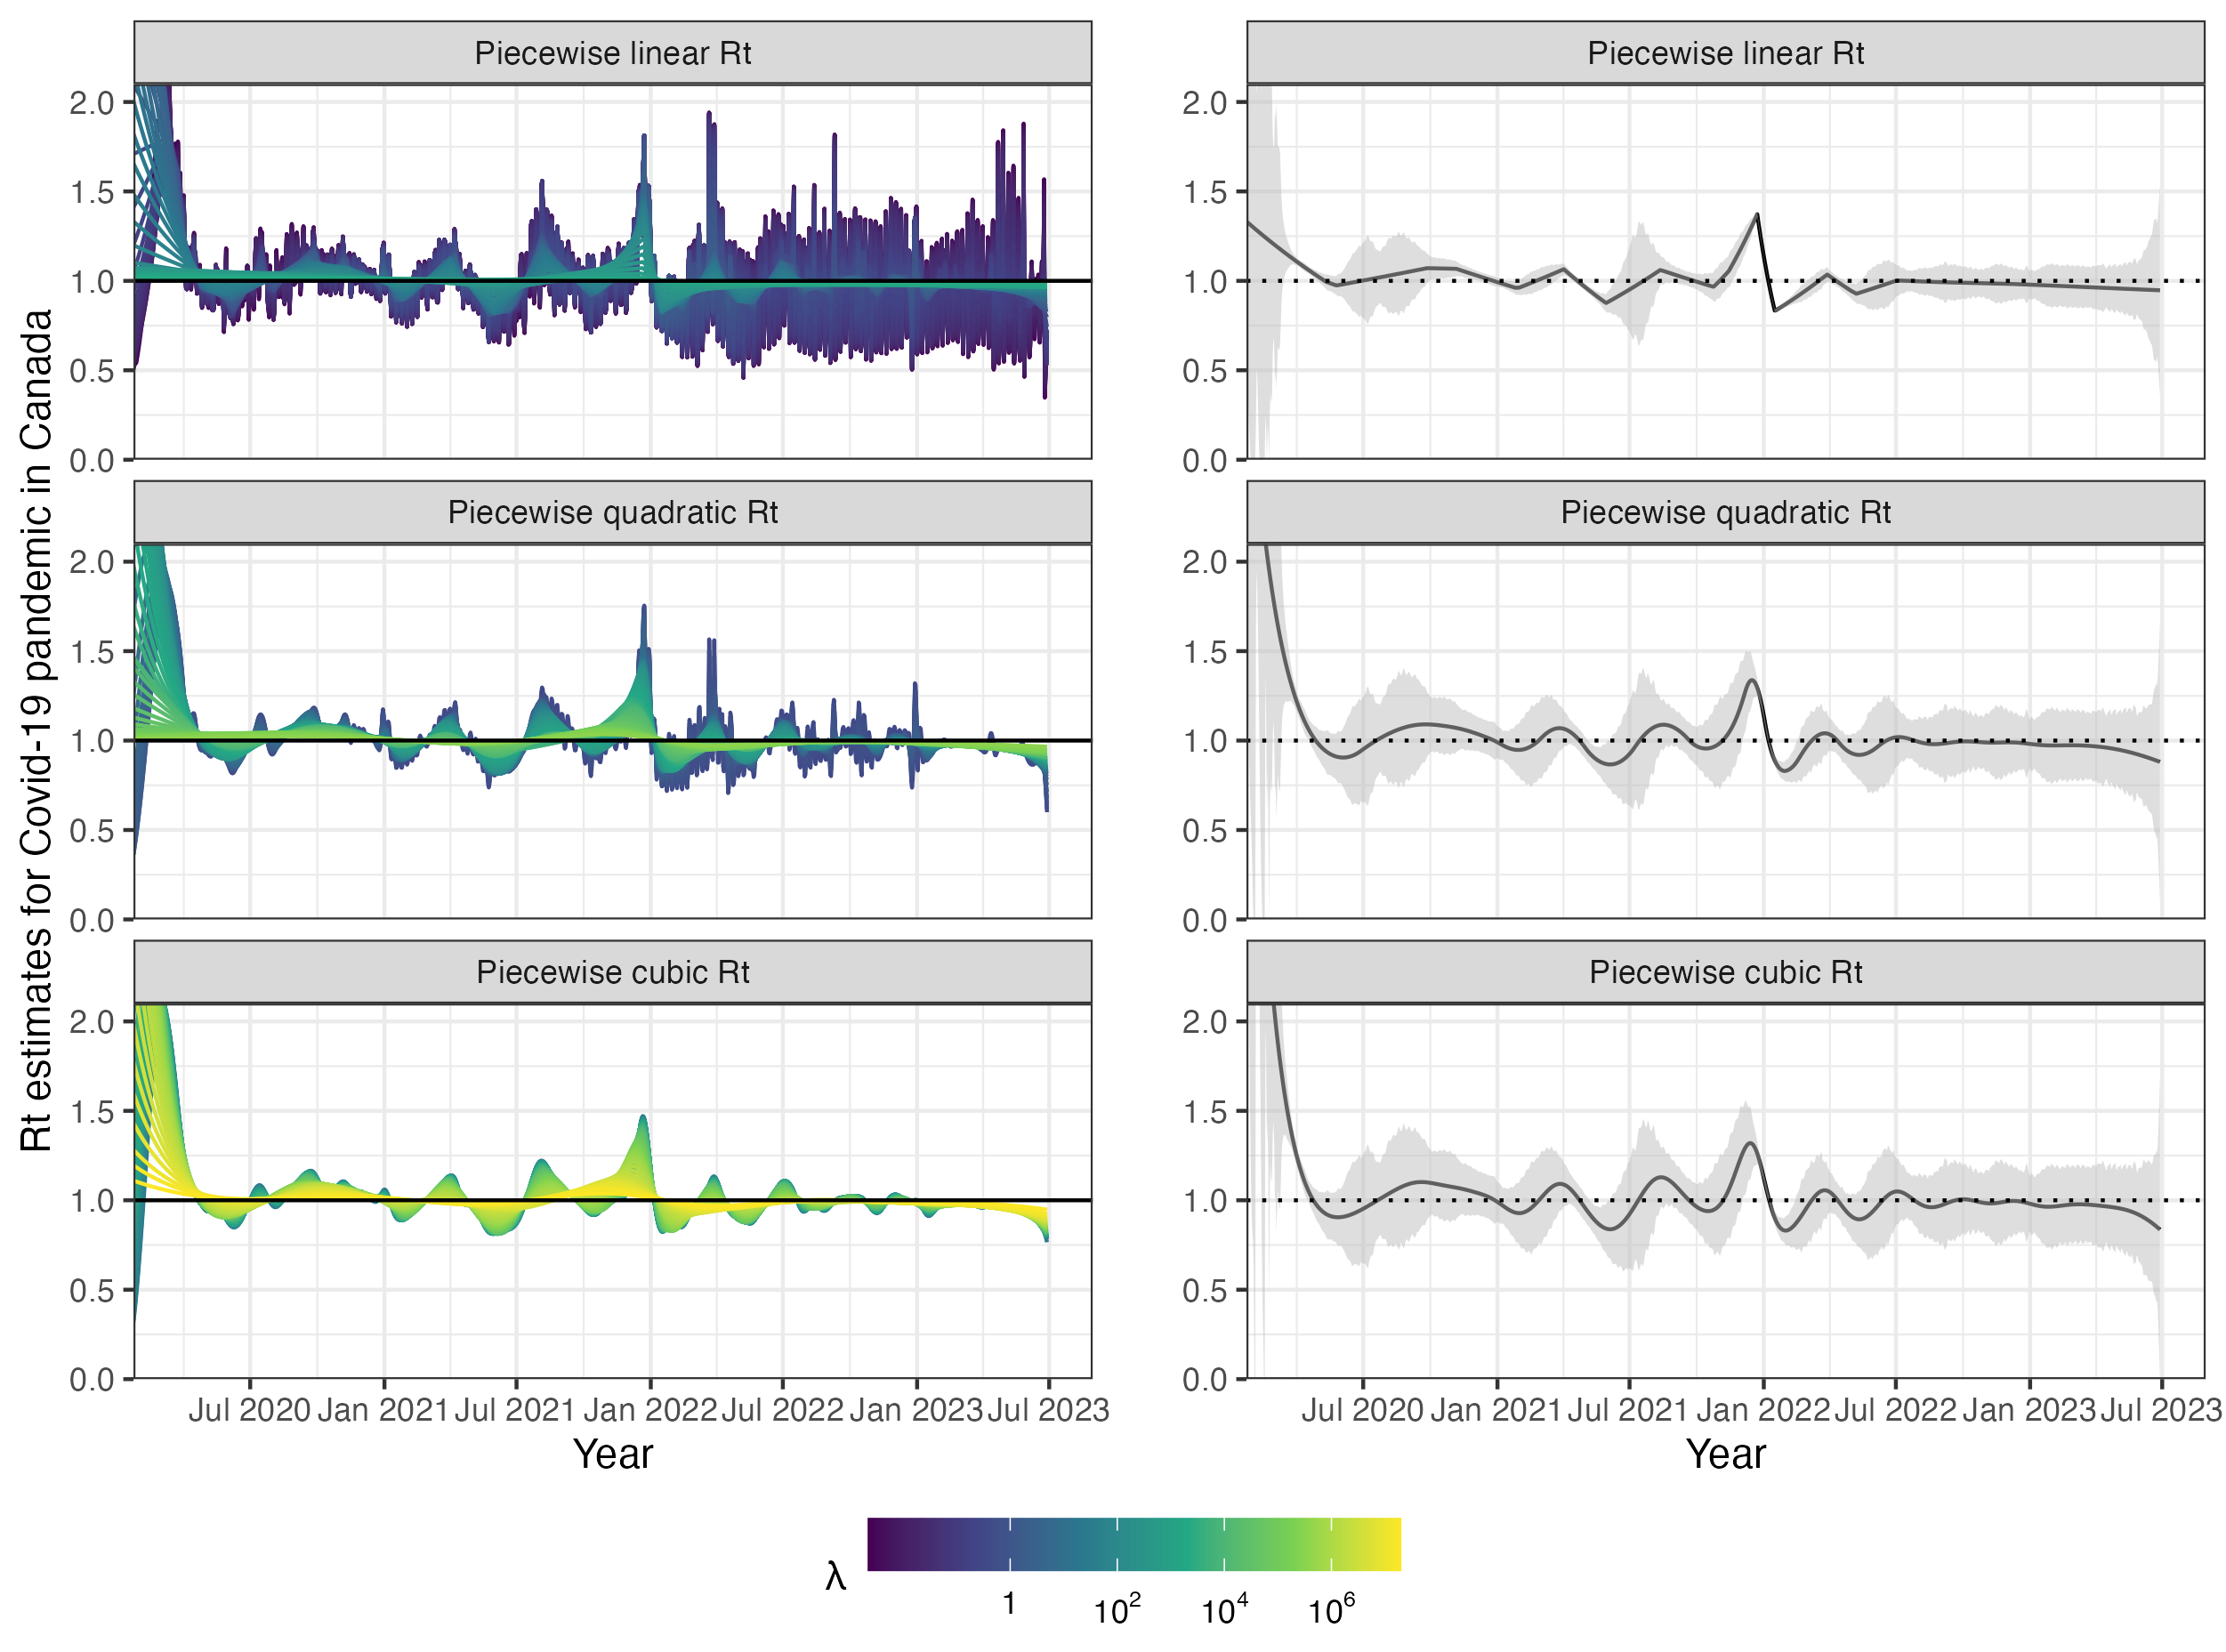
\includegraphics[width=0.9\linewidth]{fig/covid_full_res.png}
  \caption{Estimated effective reproduction number based on Covid-19 daily
  confirmed incident cases between March 1st, 2020 and April 15th, 2023 in
  British Columbia, Canada. The left panels show estimates corresponding to 50
  tuning parameters. The right panels show the CV-tuned estimate along with
  approximate 95\% confidence bands. The top, middle and bottom panels show the
  estimated $\calR_t$ using the Poisson trend filtering in \eqref{eq:rt-ptf}
  with degrees $k=1,2,3$ respectively.} 
  \label{fig:covid-rt}
\end{figure} 

The estimated effective reproduction numbers are relatively unstable before April,
2022. The highest peak coincides with the emergence and global spread of the
Omicron variant. The estimated effective reproduction numbers fall below 1 during two time
periods---roughly from April, 2021 to July, 2021 and from January,
2022 to April, 2022. The first trough coincides with the introduction of
Covid-19 vaccines in British Columbia. The second trough, shortly after the
largest peak may be due to variety of factors resulting in the depletion of the
susceptible population such as increased self-isolation in response to media
coverage of the peak or immunity incurred via recent infection. Since April,
2022, the estimated effective reproduction number has remained relatively stable
(fluctuating around one) corresponding to low reported cases, though reporting
behaviours also changed significantly since the Omicron wave. 


\subsection{Real-data results: influenza in Baltimore, Maryland, 1918}

We also apply \RtEstim\ to daily reported influenza cases in Baltimore, Maryland
occurring during the world-wide pandemic of 1918 from September to November 
\citep{frost1919influenza}. 
The data, shown in \autoref{fig:flu-dat}, is included in the \EpiEstim\ \R\ package.
The 1918 influenza outbreak, caused by the H1N1 influenza A virus, was
unprecedentedly deadly with case fatality rate over 2.5\%, infecting almost
one-third of the population across the world \citep{taubenberger20061918}. The
CV-tuned piecewise cubic estimates in \autoref{fig:flu-res} better capture the
growth at the beginning of the pandemic in \autoref{fig:flu-dat}. The estimated
$\calR_t$ curve suggests that the transmissibility of the pandemic grew rapidly
over the first 30 days before declining below one after 50 days. However, it
also suggests an increase in infectiousness toward the end of the period. With
this data, it is difficult to determine if there is a second wave or a steady
decline ahead. The CV-tuned piecewise constant and linear estimates in
\autoref{fig:flu-res} both suggest a steady decline. This conclusion is
supported by the fact that incident cases decline to zero at the end of the
period and matches $\calR$ estimates in \cite{cori2013new}, which are all lower
than one.

\begin{figure}[!ht]
  \centering
  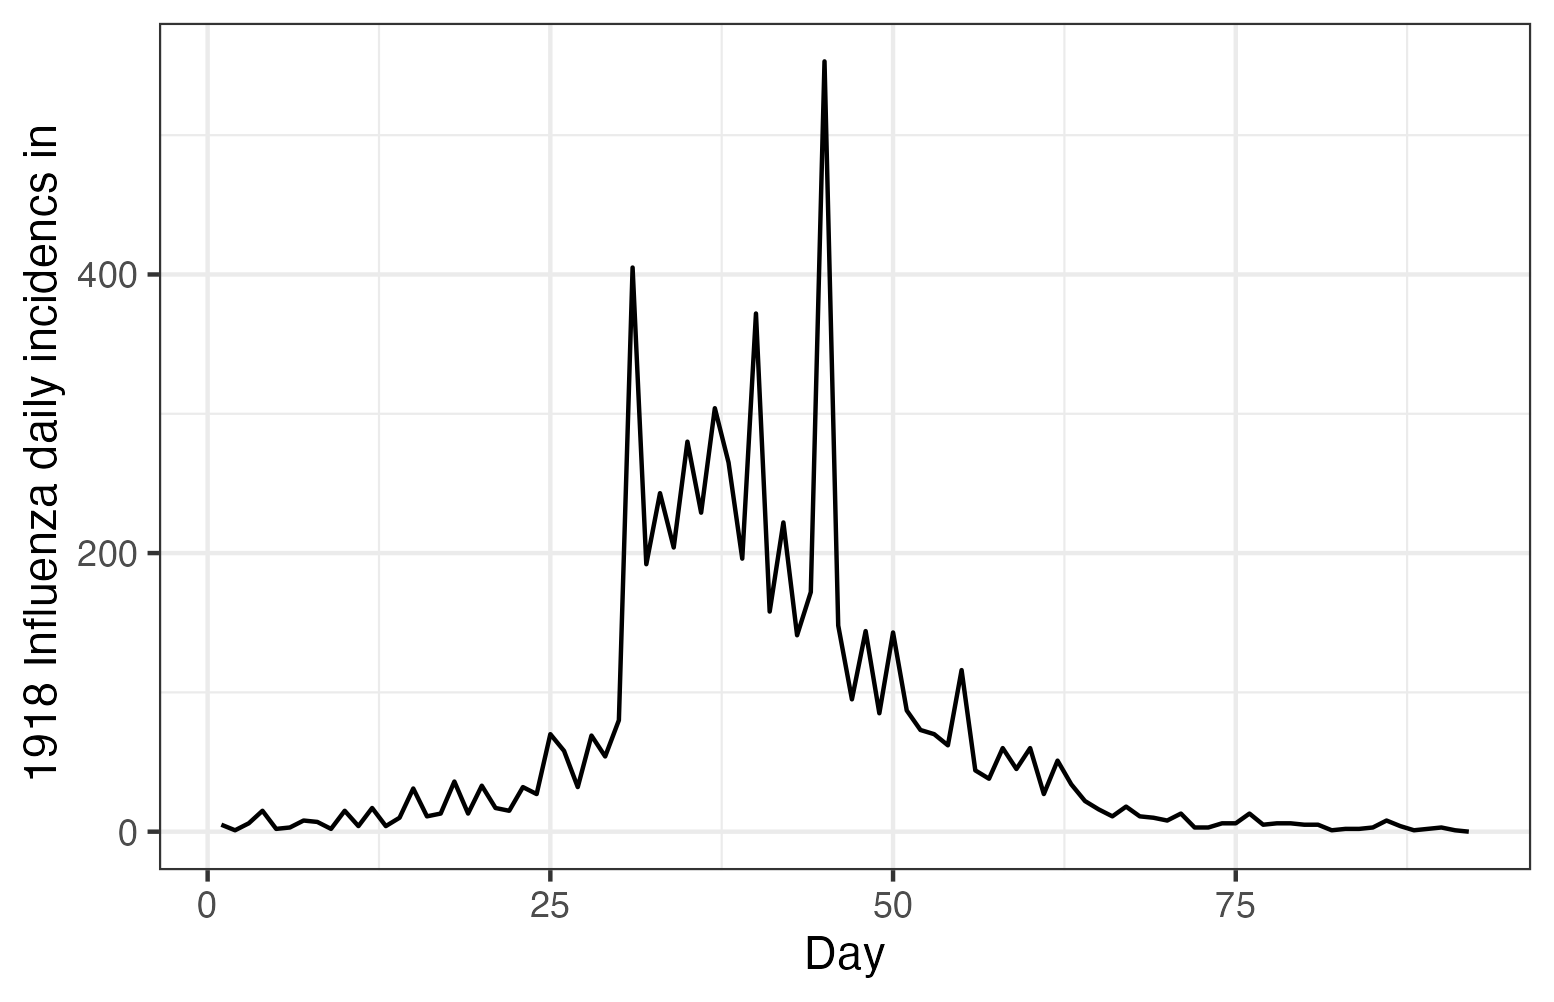
\includegraphics[width=0.9\linewidth]{fig/flu_dat.png}
  \caption{Daily incident influenza cases in Baltimore, Maryland between September 
  and November in 1918.} 
  \label{fig:flu-dat}
\end{figure} 

\begin{figure}[!ht]
  \centering
  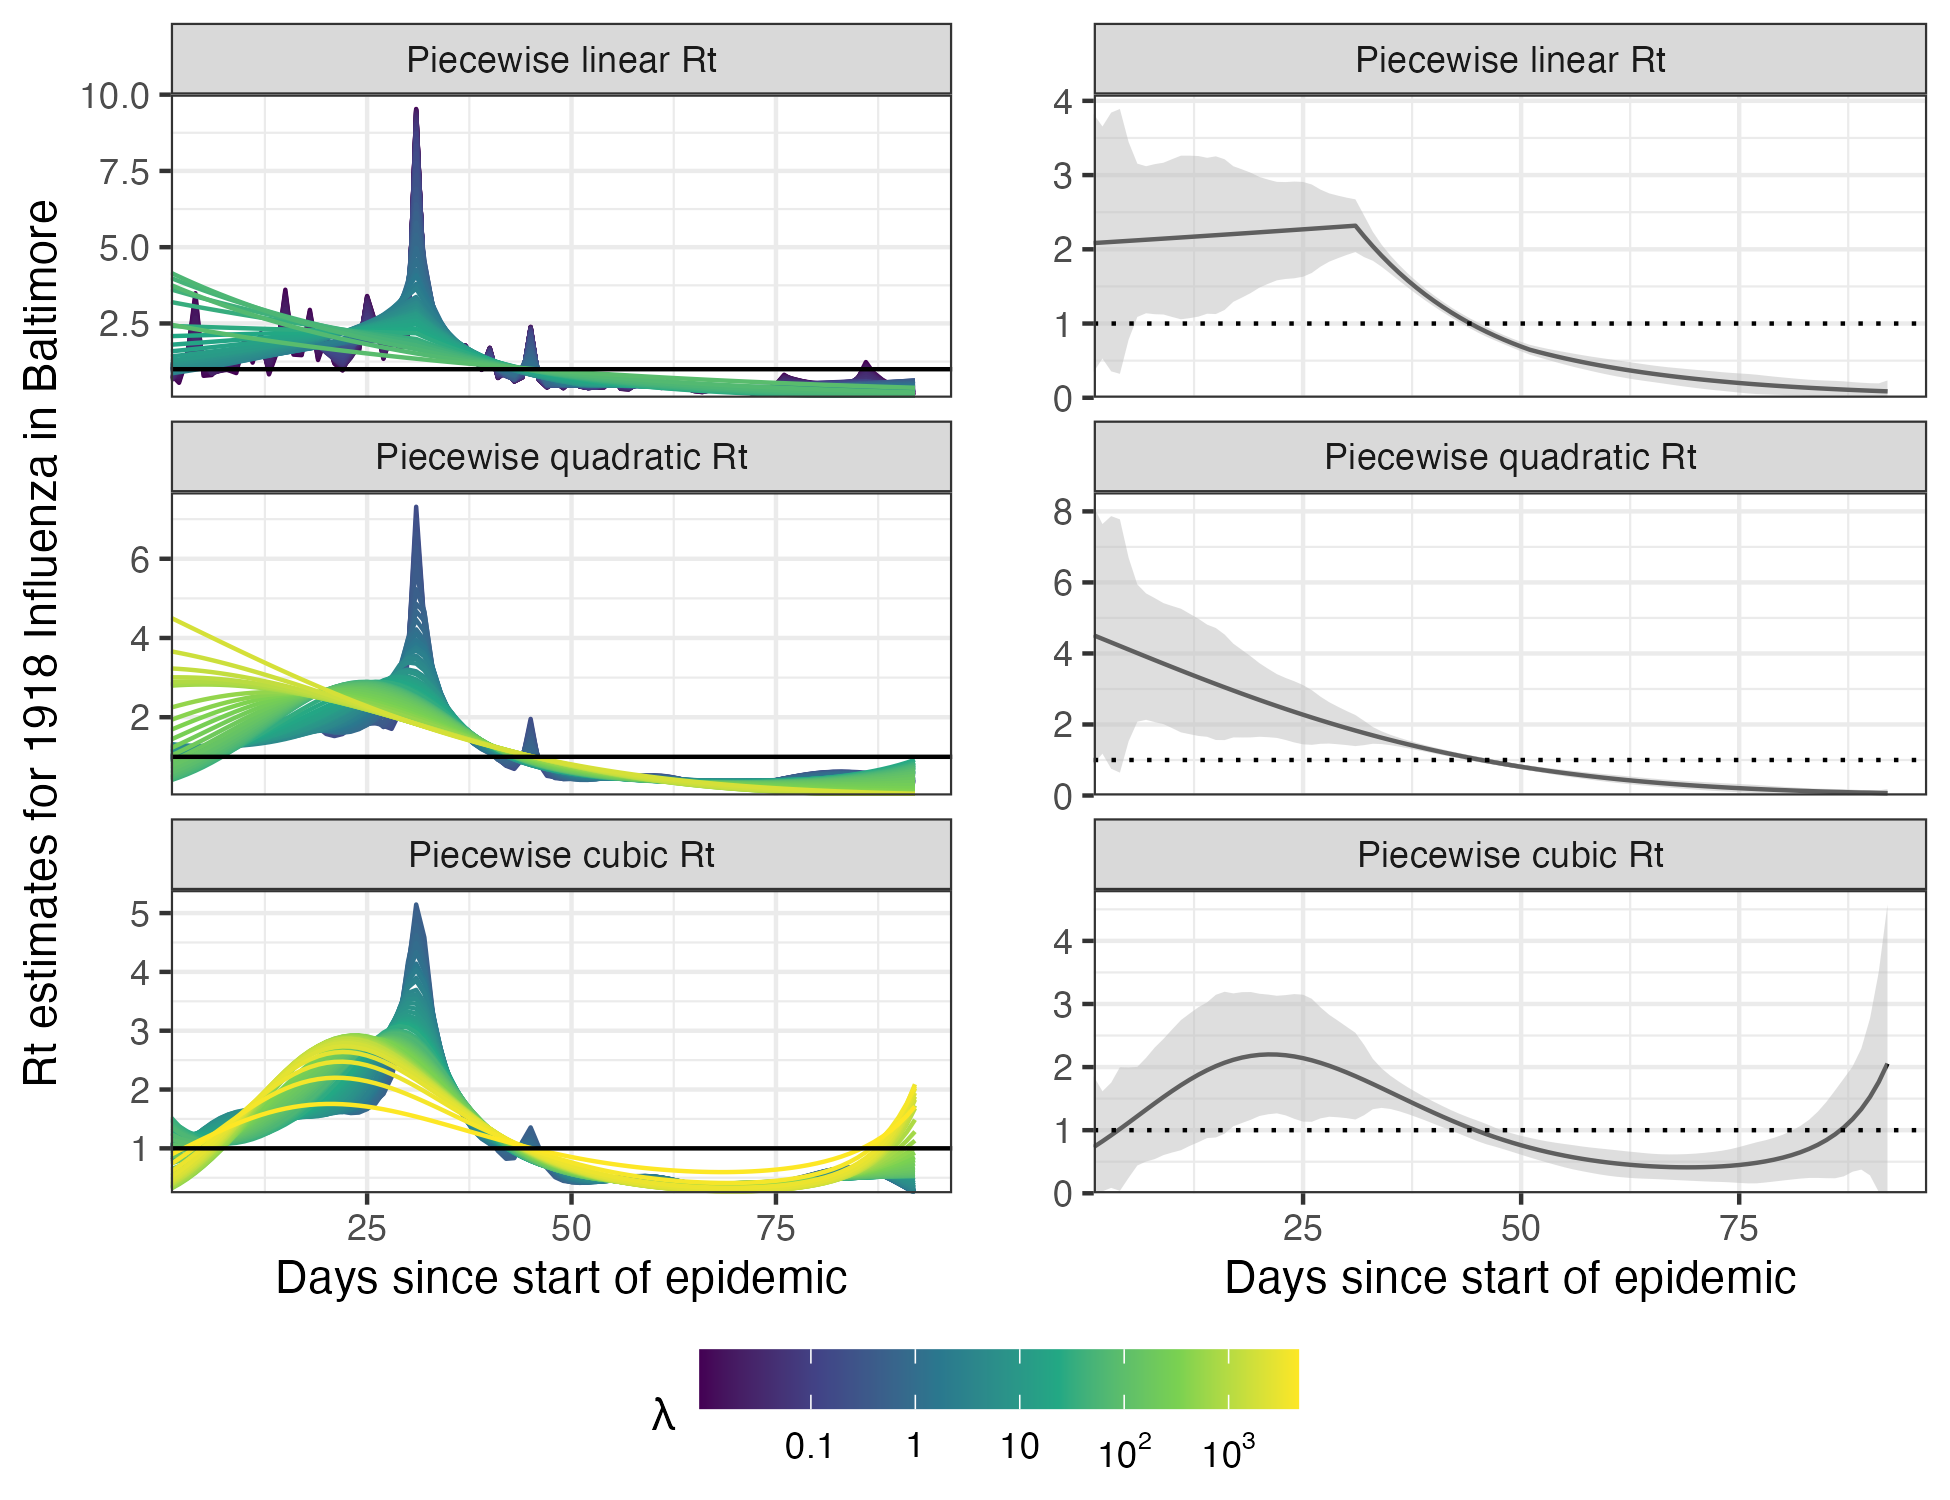
\includegraphics[width=0.9\linewidth]{fig/flu_full_res.png}
  \caption{Estimated effective reproduction numbers for influenza in Baltimore,
  Maryland in 1918. The left panels show estimates for a set of 50 tuning
  parameters. The right column displays the CV-tuned estimates with approximate
  95\% confidence bands. The rows (top to bottom) show estimated effective reproduction
  numbers ($\calR_t$) using the Poisson trend filtering in \eqref{eq:rt-ptf}
  with $k=1,2,3$ respectively.} 
  \label{fig:flu-res}
\end{figure} 
